\documentclass[a4paper,12pt]{article}
\usepackage{anysize}
\marginsize{3cm}{3cm}{1cm}{3cm}
\usepackage{amsmath}
\usepackage{amsthm}
\usepackage{bbm}
\usepackage{graphicx}

\begin{document}
\title{\textbf{Computational Statistics: Homework 3}}
\author{Michal Porvaznik \\ Nemesis key = e7e6504}
\date{March 17, 2015}
\maketitle
%
\section*{Exercise 1}
%
a) We can see from the graph below that bias is is an increasing function of the $m''(x)$. However, this is not theoretically clear from the lecture materials. The bias is also highest at the boundary.

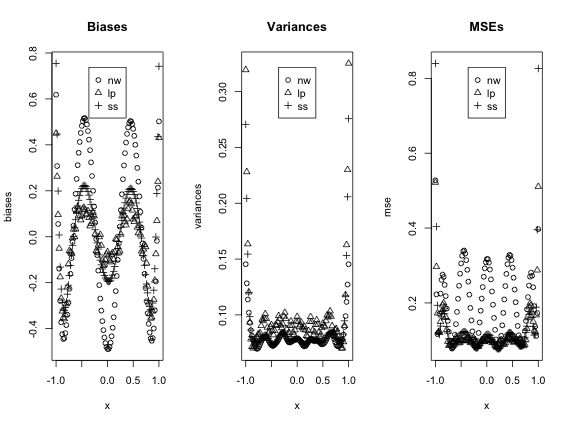
\includegraphics[scale = 0.75]{hmw3_plot1.png}

I also wanted to check the bias-variance decomposition of the mean squared error. In theory we expect that $MSE(\hat{m}(x)) = bias(\hat{m}(x))^2 + variance(\hat{m}(x))$, however in the plot below we see that this breaks down, especially near boundaries. Why is this? Are the bias/variance estimates inaccurate near the boundary? If so, why?

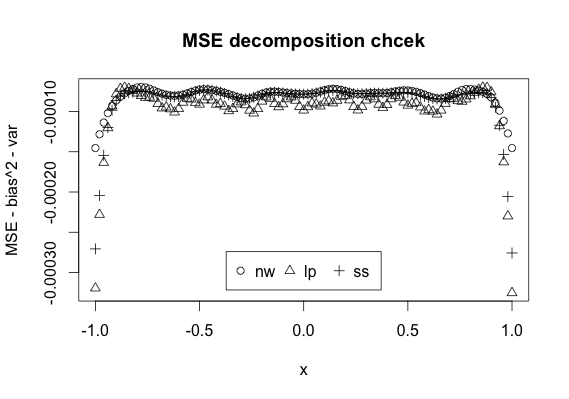
\includegraphics[scale = 0.75]{hmw3_plot2.png}

b) Upon calculating the standard error estimates and looking at the bias adjusted 95\% confidence interval $I(x) = \hat{m}(x) \pm 1.96 \cdot \widehat{s.e.}(\hat{m}(x)) - \widehat{bias}(\hat{m}(x))$, I observed the following coverage rates. For $I(0.5)$, I observed 98.3\%, 96.7\% and 97.5\% coverage rates for the Nadaraya-Watson, Local Polynomial and Smoothing Splines respectively.  The corresponding confidence bands, that is proportions of simulations where estimates at all predictor points belong to its bias adjusted 95\% confidence interval, were 68.2\%, 46.7\% and 59.8\%.
\\
\\
c) In the graph below we have a plot of bias, variance and MSE estimates for non-equidistant points. The coverage rates of the adjusted confidence intervals were higher in this case. For $I(0.5)$, I observed 98.8\%, 97.8\% and 99.9\% coverage rates for the Nadaraya-Watson, Local Polynomial and Smoothing Splines respectively.  The corresponding confidence bands, that is proportions of simulations where estimates at all predictor points belong to its bias adjusted 95\% confidence interval, were 81.7\%, 72.4\% and 92.7\%.

I don't really understand the effect of changing point distribution on prediction quality, and it does not seem correct to compare these two results considering different smoothing parameters of the estimators. How did you choose the smoothing parameters?

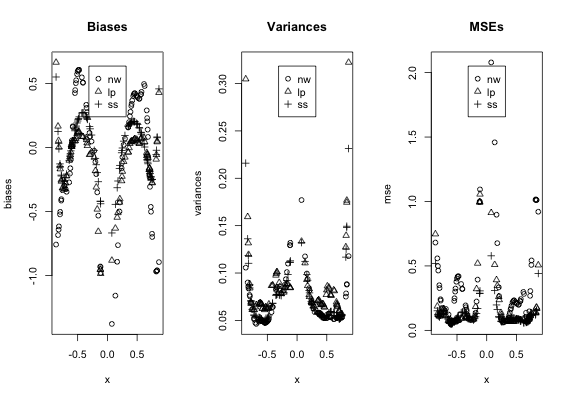
\includegraphics[scale = 0.75]{hmw3_plot3.png}

\end{document}

